\section{Základy}

V této části se podíváme na vstupní zarušený signál, který nám byl přiřazen a jeho vlastnosti.

\begin{figure}[H] 
    \centering
    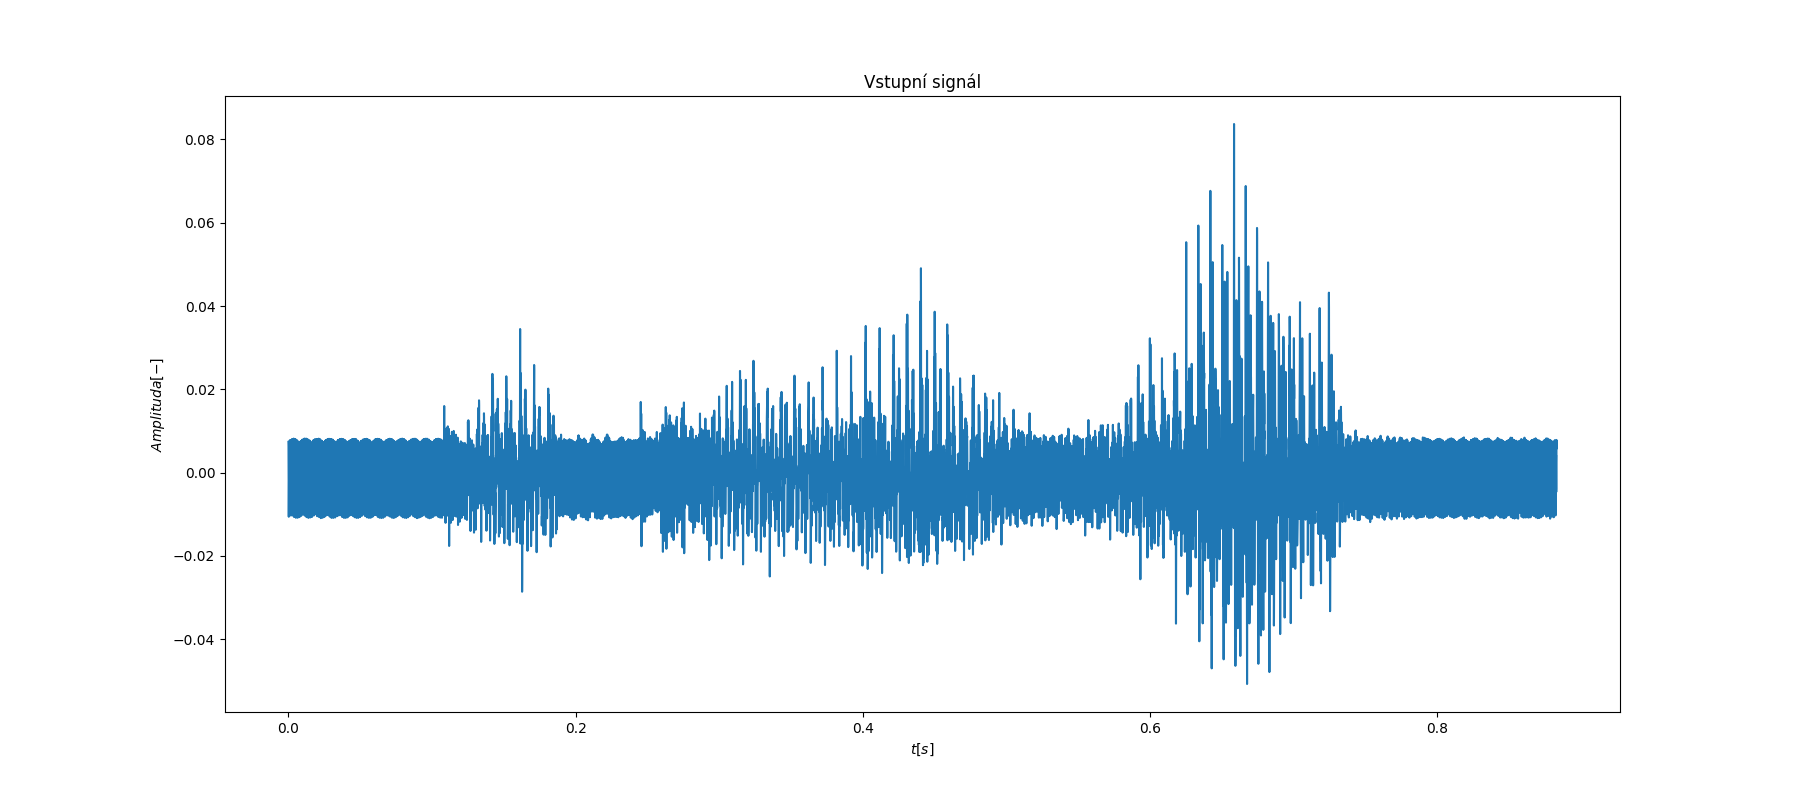
\includegraphics[scale=0.35,keepaspectratio]{Figure_1}
    \caption{Načtený signál}
\end{figure}

Délka vstupního signálu je 14132 vzorků což při vzorkovací frekvenci 16kHz odpovádá 0.88325s.
Maximální hodnota tohoto signálu je přibližně 0.837097 a minimální přibližně -0.050751.